\documentclass{article}
\usepackage[utf8]{inputenc}
\usepackage{amsmath}
\usepackage{verbatim}
\usepackage{amsfonts}
\usepackage{graphicx}
\usepackage{listings}
%
\title{%
    2º Projeto da disciplina Estruturas de Dados II \\
     \large Análise assintótica de algoritmos de ordenação}
\author{Danillo Mendes Santiago 10414592\\Gabriel Passarelli 11218480\\ Marcelo Kenji Noda 11275359}
%
\begin{document}
%
\maketitle
%
\section{Introdução}
O propósito deste texto é analisar a complexidade de tempo de algoritmos de busca sequencial e de busca por espalhamento. Eles foram implementados na parte prática do projeto, em linguagem C de programação, e seguindo os templates fornecidos na proposta do trabalho.\par
%
O texto está dividido em seções, e há uma seção para cada algoritmo implementado. Em cada um delas, apresentamos os resultados das medições do tempo de execução de cada algoritmo, e comentamos detalhes pertinentes de nossa implementação. Nessa parte, incluímos tabelas para facilitar a visualização dos dados de tempo. Como cada medição foi realizada três vezes, as tabelas contêm também medidas de dispersão dos dados (o desvio-padrão). Por fim, há uma seção apresentando as conclusões desenhadas pelo grupo.
%
\section{Análise dos algoritmos de busca sequencial}
\subsection{Busca sequencial simples}
%
A busca sequencial básica é um algorítmo bem intuitivo e não apresenta grandes dificuldades de implementação, ela basicamente percorre os indices da lista em ordem crescente e, a cada iteração, verifica se o indice atual comporta o elemento buscado. Nossa implementação percorre diretamente o vetor com os dados fornecidos, sendo necessário portanto o conhecimento do tamanho do vetor previamente.
A eficiência do algorítmo é linear pois ele itera sobre a quantidade de elementos no vetor.
%
\subsection{Busca sequencial com método \textit{mover-para-frente}}
%
Nesta variação o objetivo é criar uma busca auto-organizante, para facilitar proximas buscas ao longo do tempo. Para este método, isso se dá ao mover os elementos mais buscados ao início da fila.
Assim como a busca simples, é de fácil implementação e não requere memória extra, para fazê-lo itera-se por todo vetor e caso encontre o elemento, move-o para o início do vetor, portanto é garantido eficiência linear no pior caso.
O método de mover para frente gera ótimas respostas para buscas repetitivas porém não é muito seletivo, isso significa que ela pode priorizar nós pouco frequentes tanto como nós corriqueiros.
No caso médio, cada item tem probabilidade $1/n$ de ser acessado, a ordenação dos elementos é irrelevante então a complexidade média é $T(n) = 1/n + 2/n + 3/n + ... + n/n = (1 + 2 + 3 + ... + n)/n = (n+1)/2$, porém conforme é ordenada pelo uso a eficiência aumenta drasticamente.
%
\subsection{Busca sequencial com método de \textit{transposição}}
%
A busca sequencial com o método de transposição foi realizado de forma semelhante ao método de mover-para-frente, sendo que a principal diferença é a mudança de posição do elemento encontrado para a posição anterior ao invés da posição inicial.De forma similar ao método mover-para-frente, essa busca é possui maior eficiência para problemas em que as buscas por um mesmo elemento occorrem com maior frequência.
%
\subsection{Busca sequencial com índice primário}
%
Primeiramente, para que fosse possível executar a busca sequencial com índice primário foi necessário ordenar o vetor com as entradas. Para isso, foi utilizada a função "qsort" da biblioteca C. Em seguida, a tabela de índice primário,no caso do problema, um vetor de inteiros, foi criada com o tamanho $T=\frac{50000}{10000}=5$. A tabela de índices armazenou os elementos das posições múltiplas de T do vetor de entradas, de forma que o dividisse em buckets.

Uma função auxiliar para "encontrar o bucket" foi implementada, ela recebe como parâmetro a tabela de índices e o elemento procurado, a partir desses dois elementos, ela retorna o bucket correspondente do elemento, caso esse exista.

Por fim, caso exista um bucket no qual o elemento possa estar contido, é realizado uma busca dentro desse espaço.
%
\section{Análise dos algoritmos de busca por espalhamento}
Antes de irmos para a análise de cada implementação, faremos um comentário pertinente aos três exercícios, mas em especial ao primeiro e ao terceiro. Como bem se vê na \textit{main}, ao mesmo tempo em que realizamos a medição do tempo de inserção e a do de busca na tabela de hashing, contamos o número de colisões e o de itens encontrados, respectivamente. Contudo, isso não prejudica nossa análise comparativa dos diferentes hash's, pois, além dos custos dessas operações serem bem inferiores ao custo das operações de nosso interesse, elas incrementam na mesma porção o tempo medido em cada caso.
\subsection{Hash com \textit{overflow progressivo}}
Para implementar o hashing com o método de overflow progressivo para tratamento de colisões, utilizamos a técnica apresentada em aula. Ou seja, caso haja uma colisão na tabela durante a inserção, iniciamos um laço de iterações percorrendo as posições seguintes da tabela até achar a primeira vazia. Evidentemente, se nesse processo acharmos o próprio elemento que estamos tentando inserir, o método é finalizado.\par
Note que, em nossa implementação, uma posição é vazia se ela vale \textit{NULL}. Só há dois estados possíveis para uma posição de nossa tabela: vazia ou ocupada. Não temos um indicador para posições que já fora utilizadas, porque não fazemos remoções de elementos durante a execução do código. Contudo, como sabemos que nossas entradas não têm caracteres especiais, poderíamos facilmente ter implementado uma função de remoção apenas se utilizando de uma String "sinalizadora" com caracteres especiais para indicar posições cuja entrada já foi apagada uma vez.\par
Além disso, um último detalhe sobre a implementação é que quem utilizar o hash escolherá a função de hash que irá querer através de um parâmetro passado para o construtor do hash. Quando uma função de busca ou inserção é chamada na função \textit{main}, um teste é realizado por tal função para saber qual a função de hash deve ser utilizada. Isso incrementa o custo de realização da operação em $1$, que é o custo de teste. Contudo, simplifica o uso das funções implementadas.\par
Na tabela abaixo, vemos as medições de tempo para as operações de busca e inserção, além do número de colisões. Podemos, através dela, que a função de hash h\_div se adequou melhor aos dados com que trabalhamos, pois o número de colisões na tabela quando preenchida com ela é bem inferior ao que se obtém com a h\_mul. Isso, por sua vez, se reflete, como esperado, no tempo de inserção e no de busca: a h\_div foi cerca 4 vezes mais eficiente na hora de inserir elementos na tabela, e cerca de 3 vezes na hora de realizar buscas. Por fim, o valor pequeno no desvio-padrão indicar a consistência de nossas medidas.
\begin{table}[h!]
    \begin{tabular}{c|c|c|c}
         & Inserção & Busca & Colisões \\ 
        \hline
        h\_div & $\mu = 1.32\cdot 10^{-1},\;\sigma = 4.9\cdot10^{-4}$ & $\mu=3.29\cdot 10^{-1},\;\sigma = 3.36\cdot 10^{-3}$ & 25461 \\
        \hline
        h\_mul & $\mu=4.08\cdot10^{-1},\;\sigma=4.25\cdot 10^{-3}$ & $\mu=9.4\cdot 10^{-1},\;\sigma=3.33\cdot 10^{-3}$ & 33959\\
        \hline
    \end{tabular}
    \caption{Medidas de tempo e do número de colisões em cada hash. $\mu$ indica a média das medidas e $\sigma$, o desvio padrão. Todas as medidas estão em segundos.}
\end{table}\par
%
%
%
\subsection{Hash com \textit{hash duplo}}
A implementação desse exercício foi um pouco mais simples do que a do anterior. Isso porque agora só fizemos as medições de tempo para uma função hash. Em relação ao anterior, vemos que o número de colisões foi muito parecido com o da função de hash hash\_mul sozinha, o que não é estranho, já que a função de hash nesse caso está altamente relacionada à hash\_mul, evidentemente. Contudo, vemos que o tratamento da colisão é mais eficiente agora do que antes, pois o método de hash duplo tem medidas de tempo inferiores tanto na inserção dos dados quanto na busca. Essa maior eficiência se deve à capacidade desse método de distribuir mais uniformemente os dados.
\begin{table}[h!]
    \begin{tabular}{c|c|c|c}
         & Inserção & Busca & Colisões \\ 
        \hline
        h & $\mu = 1.90\cdot 10^{-1},\;\sigma = 8.30\cdot10^{-3}$ & $\mu=3.89\cdot 10^{-1},\;\sigma = 3.44\cdot 10^{-3}$ & 33960 \\
    \end{tabular}
    \caption{Medidas de tempo e do número de colisões no hash duplo. $\mu$ indica a média das medidas e $\sigma$, o desvio padrão. Todas as medidas estão em segundos.}
\end{table}
%
\subsection{Hash aberto com lista encadeada não ordenada}
%
Neste exercício, a implementação da tabela de Hashing foi bem mais simples do que as anteriores. Contudo, a facilidade inicial foi compensada pela necessidade de se implementar uma lista encadeada. Como esperado, o número de colisões aqui é consideravelmente menor do que nos outros métodos.\par
Além disso, as operações de busca e de inserção também são mais eficientes. Isso tem a ver com o fato de que, em nossa implementação do exercício a, calculamos a representação inteira da palavra a ser inserida ou buscada a cada nova iteração do for que percorre a tabela de hashing (guardar o valor em uma variável e utilizá-lo a cada novo laço seria uma forma de otimizar o código, portanto), e também com o fato de que na lista encadeada o número de iterações que teremos que fazer até chegar ao final da lista pode ser menor do que o número de iterações que teremos que fazer até chegar numa posição vazia da tabela da hashing. Para enxergar isso, podemos imaginar um procedimento de inserção nas duas tabelas de hashing: suponha que houve uma colisão na posição $x$ e que essa foi a primeira colisão de algum elemento com $x$; na lista encadeada, simplismente iremos inserir um novo elemento, sem ter que percorrer nenhum outro; na tabela com overflow progressivo, iremos caminhar até a próxima posição vazia, o que pode custar até B iterações.
\begin{table}[h!]
    \begin{tabular}{c|c|c|c}
         & Inserção & Busca & Colisões \\ 
        \hline
        h\_div & $\mu = 3.88\cdot 10^{-2},\;\sigma = 7.0\cdot10^{-4}$ & $\mu=6.03\cdot 10^{-2},\;\sigma = 6.3\cdot 10^{-4}$ & 28558 \\
        \hline
        h\_mul & $\mu=1.26\cdot10^{-1},\;\sigma=2.04\cdot 10^{-3}$ & $\mu=2.43\cdot 10^{-1},\;\sigma=4.33\cdot 10^{-3}$ & 34333\\
        \hline
    \end{tabular}
    \caption{Medidas de tempo e do número de colisões em cada hash. $\mu$ indica a média das medidas e $\sigma$, o desvio padrão. Todas as medidas estão em segundos.}
\end{table}\par
%
\section{Conclusão}
A figura \ref{fig:graficoresultados} apresenta o tempo médio na execução dos diferentes tipos de buscas realizadas. O tempo em questão representa apenas o tempo para o processo de busca, isso é, desconsiderando o tratamento anterior para algumas outras estruturas.

%% incluir grafico %%

\begin{figure}[!htb]
    \centering
    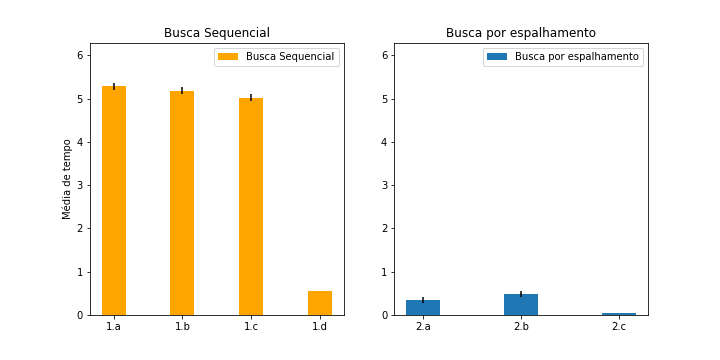
\includegraphics[width=13cm]{grafico.png}
    \caption{Resultados obtidos}
    \label{fig:graficoresultados}
\end{figure}

As tabelas \ref{tab:resultados} e  \ref{tab:resultados2} apresentam os resultados numéricos da média e do desvio padrão

\begin{table}[!htb]
    \centering
    \begin{tabular}{|c|c|c|c|c|}
    \hline
         & 1a & 1b & 1c & 1d   \\ \hline
      Média & 5.2781 & 5.1793 &  5.0190& 0.5533  \\\hline
      Desvio Padrão & 0.0853 & 0.0759 &  0.0860 & 0.0086 \\\hline
    \end{tabular}
    \caption{Tabela com resultados da Parte I}
    \label{tab:resultados}
\end{table}

\begin{table}[!htb]
    \centering
    \begin{tabular}{|c|c|c|c|}
    \hline
         & 2a   & 2b & 2c   \\ \hline
      Média & 0.3536 & 0.4864 &  0.0547 \\\hline
      Desvio Padrão & 0.0663 &  0.0616 &  0.0023\\ \hline
    \end{tabular}
    \caption{Tabela com resultados da Parte II}
    \label{tab:resultados2}
\end{table}

A partir das tabelas e dos gráficos é possível verificar uma diferença significativa entre maioria das buscas sequenciais e das buscas por espalhamento. Sendo a principal delas a busca através do método de mover-para-frente.
Além disso, é possível perceber que os métodos que realizam algum tipo de "tratamento" anterior ao processo de busca, como a busca sequencial com índice primário e as buscas por espalhamento apresentaram um desempenho melhor.
\end{document}
